\section{Tremor}
\label{section:tremor}

In dit hoofdstuk worden tremoren besproken.
Aan het einde van het hoofdstuk is het duidelijk wat een tremor is,
welke verschillende tremoren er zijn, en hoe deze geclassificeerd worden.
Hierbij zal de Essentiële Tremor (ET) extra aandacht krijgen,
gezien deze vorm van tremor centraal staat tijdens dit onderzoek.
Dit hoofdstuk geeft antwoord op de vraag: Wat is een Essentiële Tremor?

\subsection{Wat is een tremor?}

Tremoren zijn onwillekeurige bewegingsstoornissen die kunnen worden gedefinieerd als een ritmische,
trillende beweging van een lichaamsdeel\cite{knf2022}.
Iedereen heeft een fysiologische tremor. Dit zijn trillingen die ontstaan door, bijvoorbeeld, stress.
Het is een natuurlijke vorm van trillen die veranderd op basis van verschillende factoren\cite{hersenstichting2024,erasmus2022}.
Zodra er een diagnose vereist is, gaat het onder andere over ET,
Psychologische tremoren of een Parkinsons tremor\cite{elsevier2022}.

ET is veel voorkomende aandoening met een trilfrequentie tussen de 4 en 12Hz.
Over het algemeen zit de frequentie tussen de 4 en 6Hz\cite{frontiers2022}.
In vergelijking met een Parkinsons tremor, wordt ET geclassificeerd als actietremor.
Dit houdt in dat de tremor zich vooral voordoet bij beweging\cite{knf2022,frontiers2022,elsevier2022}.
Een psychologische tremor is het resultaat van psychologische processen in het brein \cite{elsevier2022}.

Zoals eerder vermeld, vallen tremoren onder bewegingsstoornissen.
Vergelijkbare aandoeningen zijn onder andere:

\begin{description}
    \item[Myoclonus] Niet-ritmische spiersamentrekkingen in handen of vingers\cite{knf2022}.
    \item[Dystonie] Aanhoudende spiersamentrekkingen die leiden tot afwijkende posities\cite{knf2022,elsevier2022,erasmus2022}.
    \item[Tics] Plotselinge, snelle, ongecontroleerde en niet-ritmische bewegingen\cite{knf2022}.
    \item[Parkinsons] Aandoening met traagheid, stijfheid en rusttremor\cite{knf2022,frontiers2022,elsevier2022,erasmus2022}.
    \item[Ataxie] Ongecoördineerd bewegen tijdens staan en lopen, of bij oogbewegingen\cite{knf2022}.
\end{description}

\subsection{Welke tremoren zijn er?}

In 2018 is er een classificatie opgesteld waarin verschillende condities waarin tremor optreedt worden benoemd\cite{knf2022}.
Deze classificatie is terug te zien in Figuur~\ref{figure:classification}.
De onderverdeling en benaming is versimpeld naar het artikel van Jolanda Schieving\cite{schieving2023}.

In de eerste stap van de classificatie wordt er onderscheid gemaakt tussen een actietremor en een rusttremor,
komt de tremor voor tijdens bewegen of in rust? Een rusttremor is onder andere kenmerkend voor Parkinsons,
waar een actietremor wijst in de richting ET\cite{elsevier2022}.

Actietremoren kunnen vervolgens worden onderverdeeld in drie soorten: houding- of postuurtremor,
statische- of isometrische tremor en bewegingstermoren.
Een houdingstremor is vooral merkbaar bij het aannemen van een bepaalde houding\cite{elsevier2022,erasmus2022}, 
een statische tremor is een tremor die ontstaat bij het aanhoudend spiergebruik, bijvoorbeeld rek- en strekoefeningen\cite{nowak2013, erasmus2022}.
Een bewegingstremor ontstaat bij verschillende soorten bewegingen\cite{elsevier2022}.

De bewegingstermoren zijn onder te verdelen in een simpele kinetische tremor, 
een intentietremor, of een taak-specifieke tremor. Bij een simpele tremor ontstaan er trillingen bij bewegen,
een intentietremor ziet de trillingen erger worden tussen intentie van een beweging en de daadwerkelijke beweging.
Een taak-specifieke tremor is vooral gebonden aan een specifieke (soort) taak\cite{erasmus2022}.

\begin{center}
    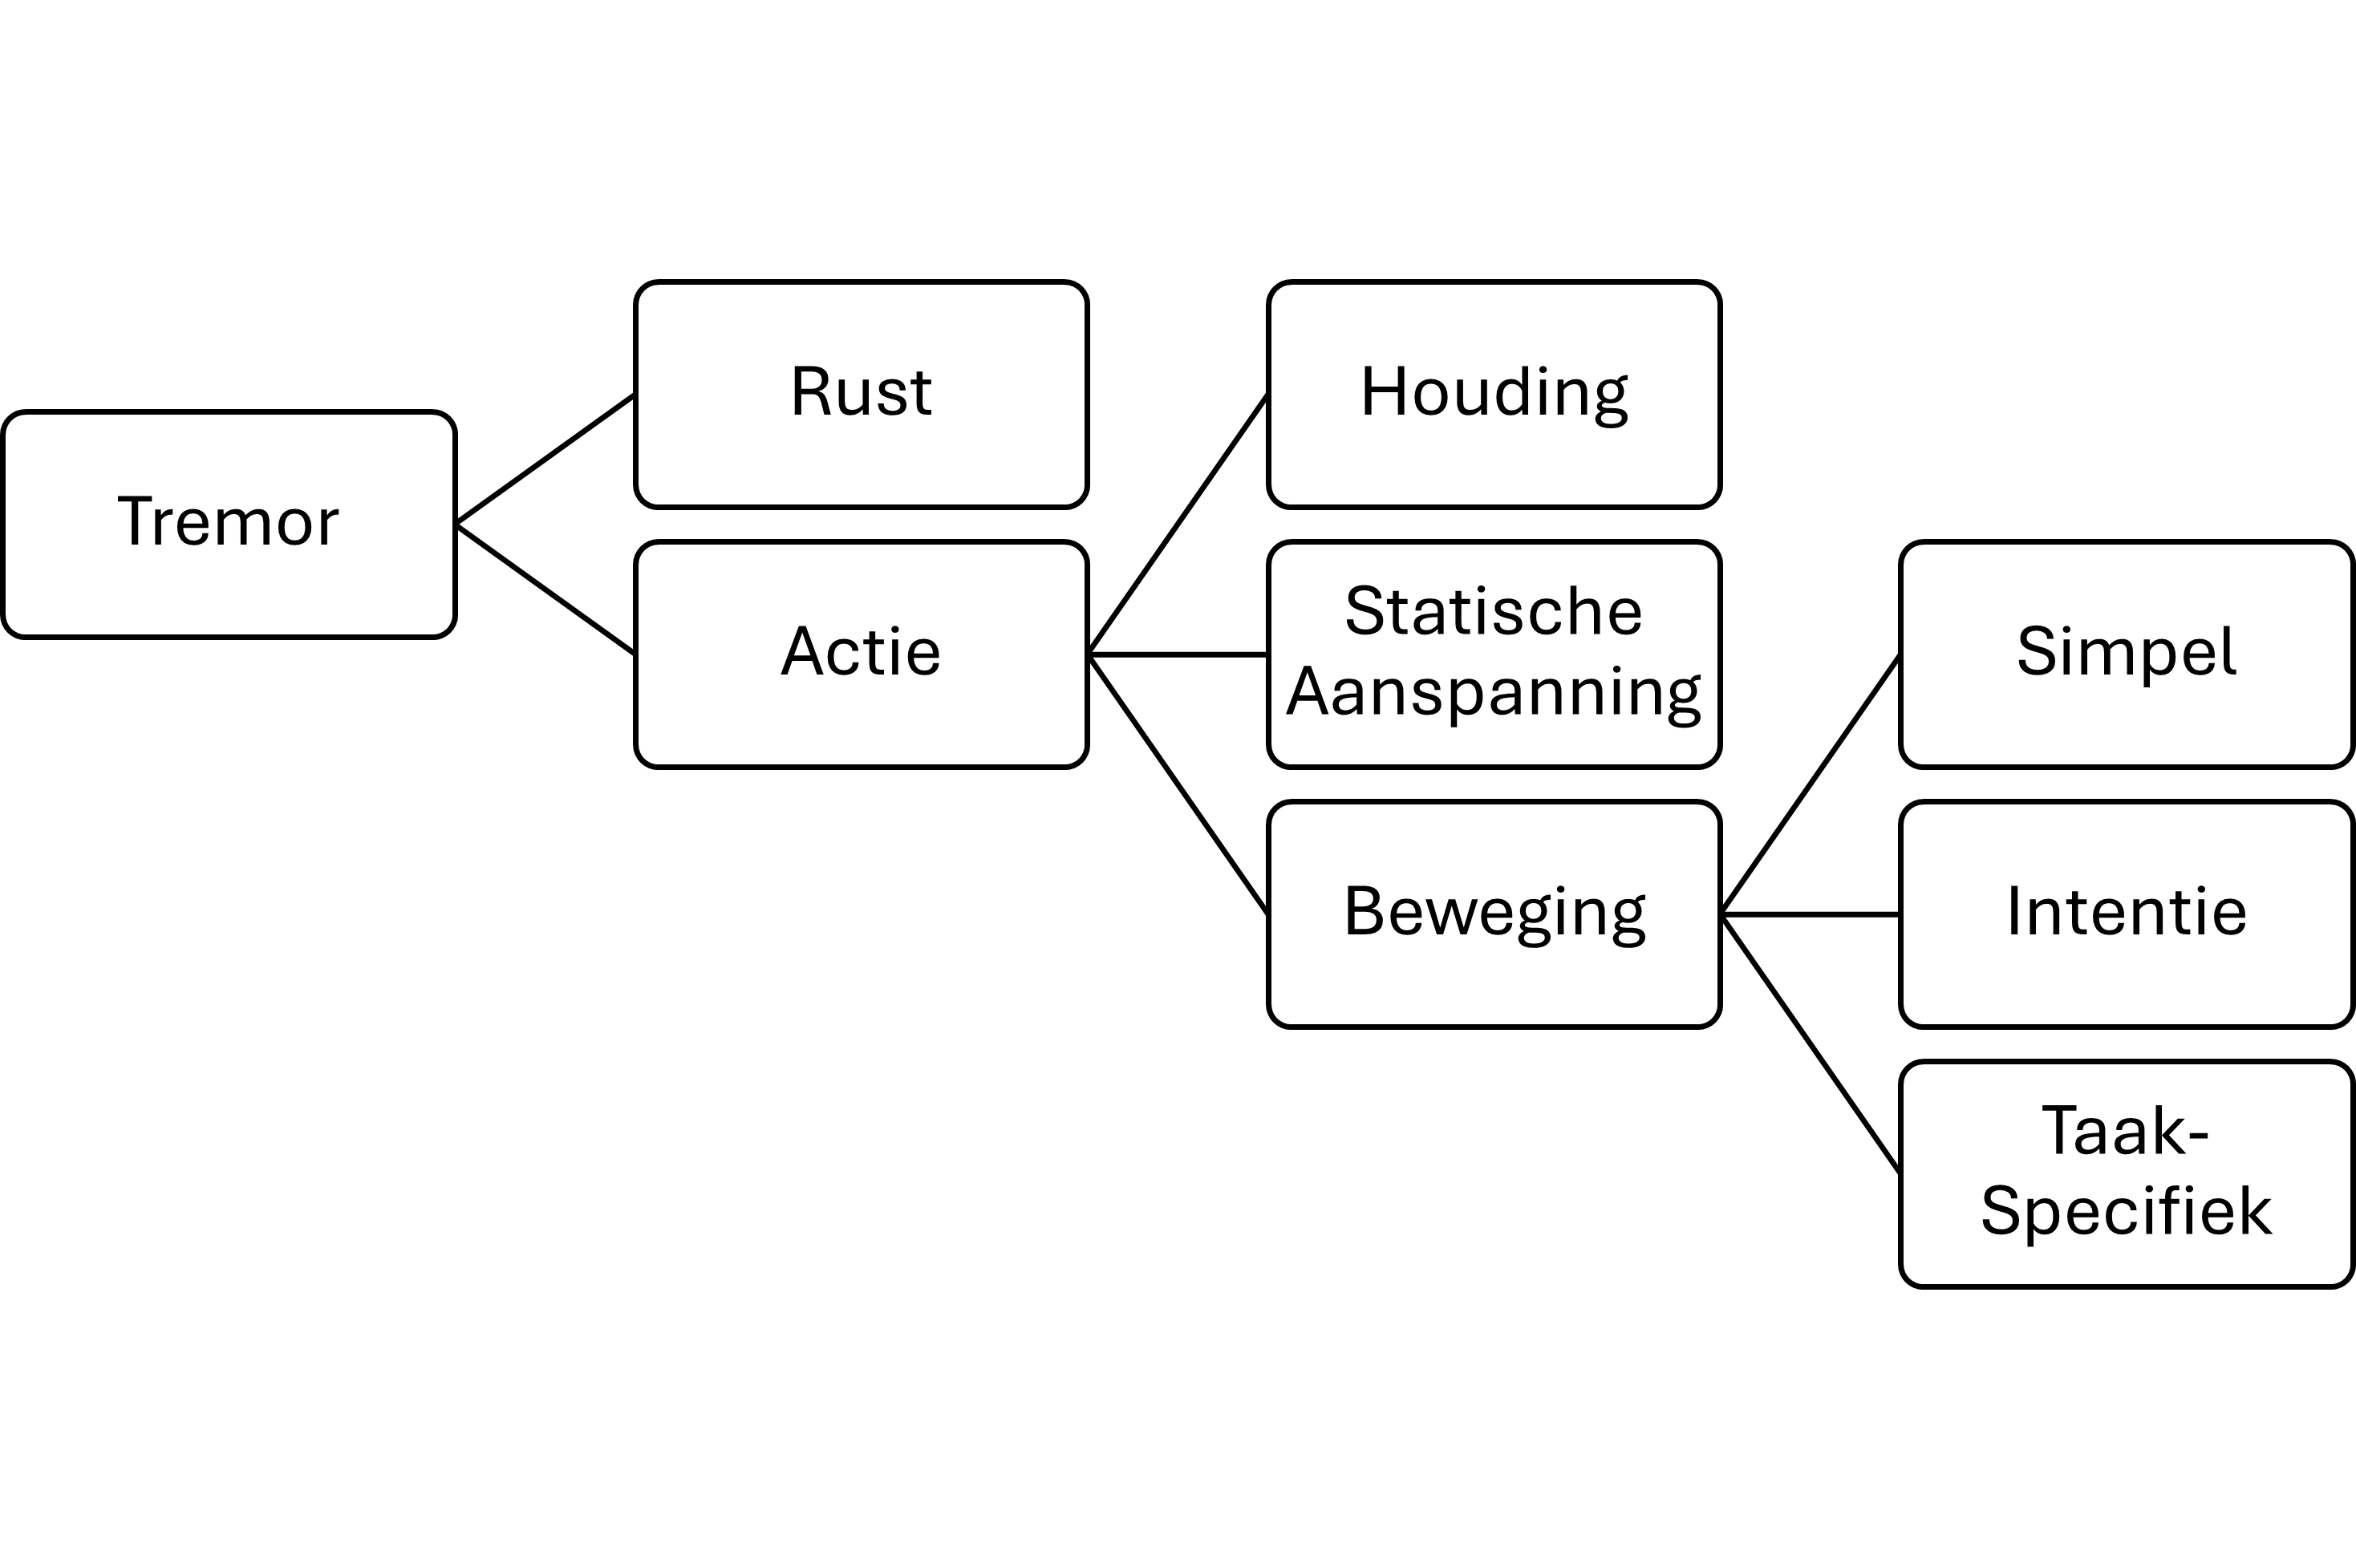
\includegraphics[width=0.4\textwidth]{./graphics/graph-tremor-classification.png}
    \captionof{figure}{Tremor Classification}
    \label{figure:classification}
\end{center}

Een uitgebreide versie van het diagram in Figuur~\ref{figure:classification}
is te vinden in de richtlijnen voor diagnose van het Erasmus MC.
Hierin zijn dezelfde classificaties te zien zoals eerder beschreven, 
met extra informatie die bedoeld is voor, naast de classificatie, de diagnose van een bepaalde tremor\cite{erasmus2022}.
Dit diagram is terug te vinden in bijlage~\ref{appendix:diagnose}.
Gezien dit onderzoek zich richt op de detectie van tremoren, is enkel de classificatie voldoende.

\subsection{Wat is een Essentiële Tremor?}